% !TEX root = main.tex

The assessment looks into the environmental impacts of production, operation, and disposal of an Adaptive Solar Facade (ASF). We assume that the ASF has a life time of 15 years.

\subsection{Life Cycle Inventory and Assumptions}

The mechanical components of the ASF can be broken into four parts: a PV panel, actuator, cantilever, and a cable net supporting structure. The PV panel, actuator and cantilever combine to form a dynamic PV module, which is then mounted on a cable net supporting structure. An exploded view of these components can be seen in Figure \ref{fig:explodedView}. There also the additional electronics which exists off the facade in a seperate control box. Theses five components are the main product systems in the manufacture of the ASF as seen in Figure \ref{fig:BOS}. 


% \begin{figure}[H]
% \begin{center}
% 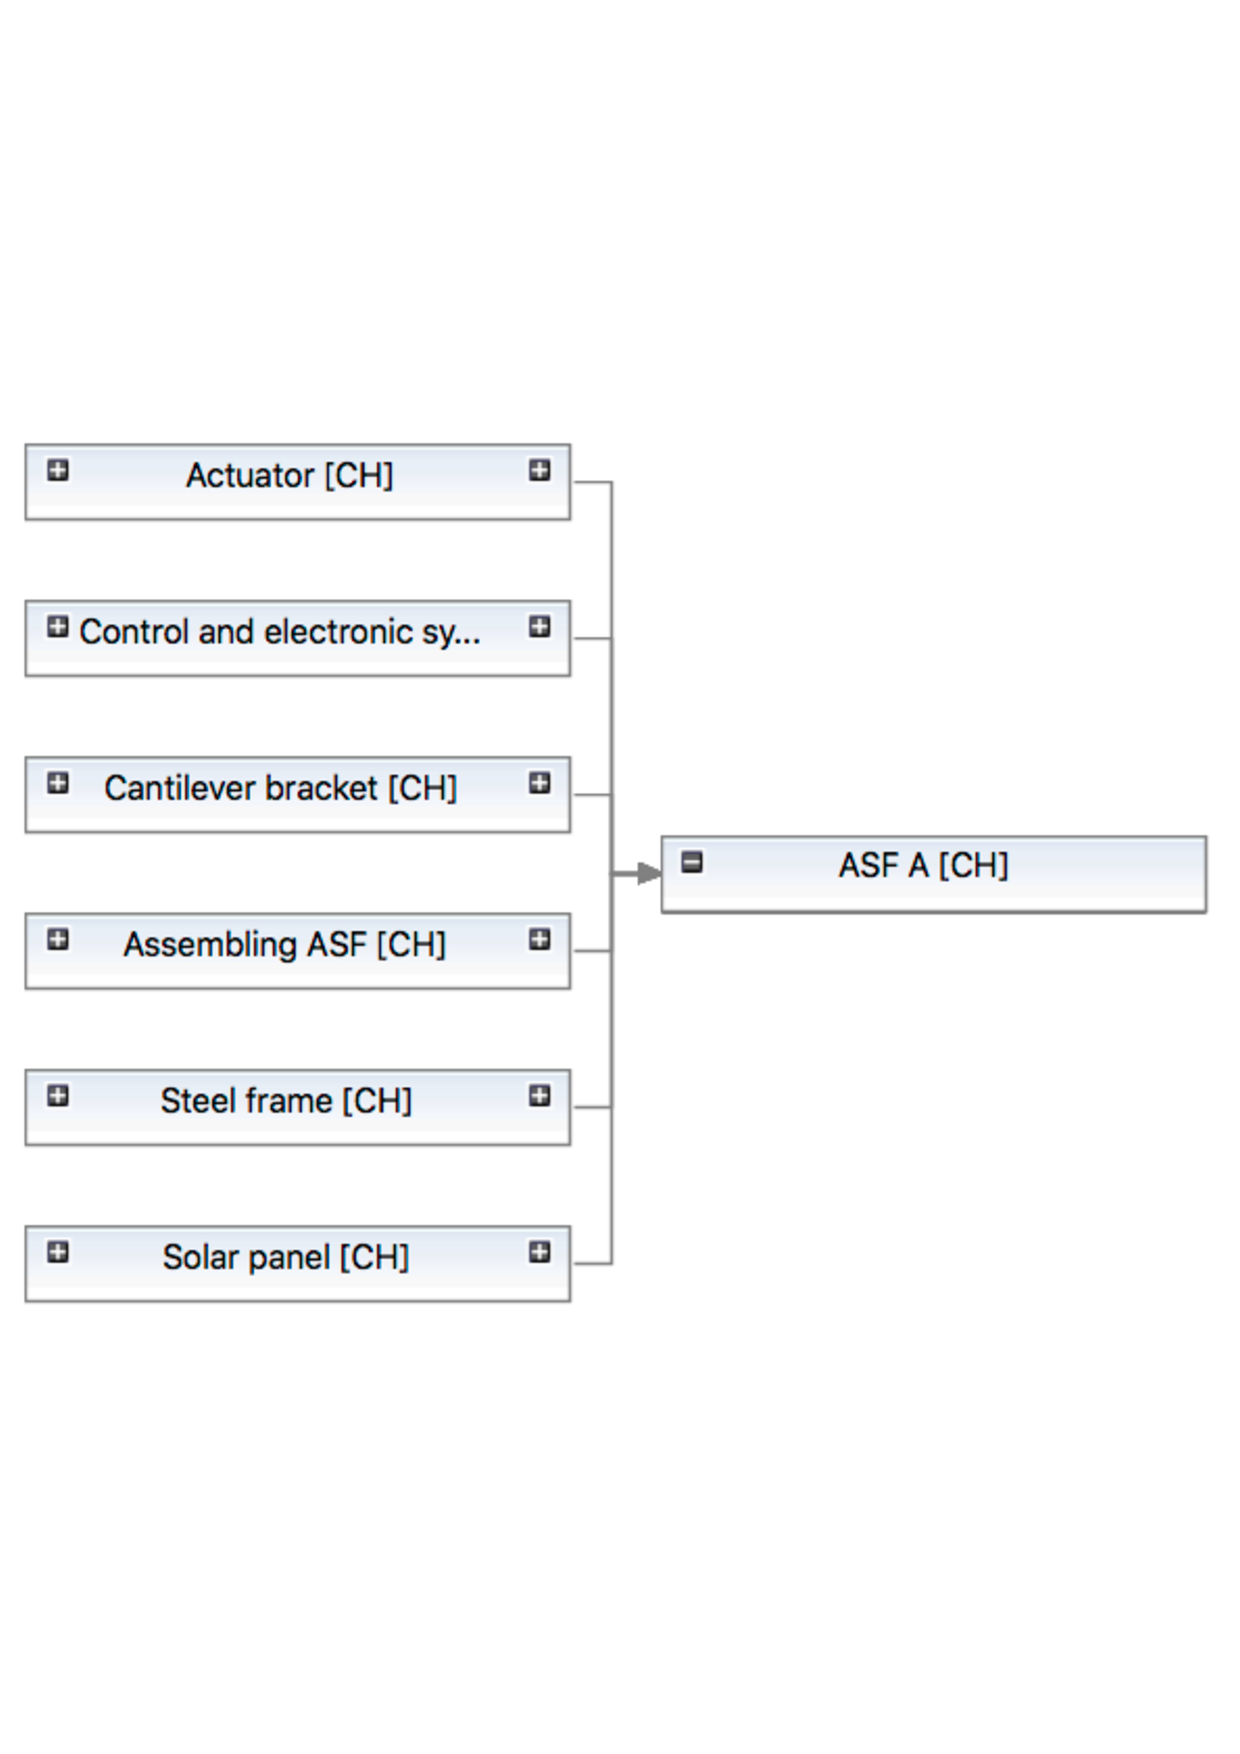
\includegraphics[width=8cm, trim= 0cm 0cm 0cm 0cm,clip]{ASFSubsystems.pdf}
% \caption{Breakdown of the ASF into six sub-product systems (Note change Steel frame to Suporting Structure, and Assembling ASF to Assembly. Also redraw this chart so it matches the subsubsections below)}
% \label{fig:subsystem}
% \end{center}
% \end{figure}

\begin{figure}[H]
\begin{center}
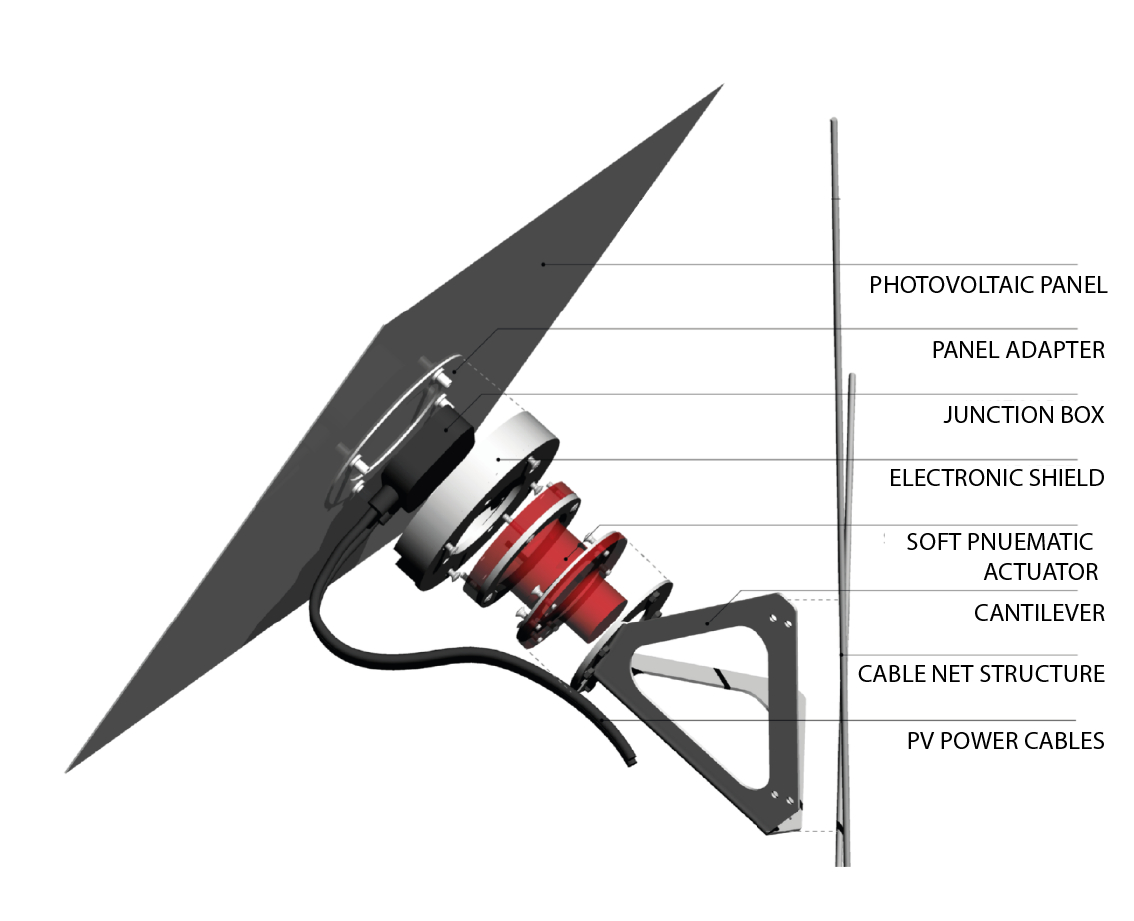
\includegraphics[width=8cm, trim= 0cm 0cm 0cm 0cm,clip]{explodedASFV2.png}
\caption{Exploded view of an ASF module mounted on a cable net supporting structure}
\label{fig:explodedView}
\end{center}
\end{figure}

\begin{figure}[ht]
\begin{center}
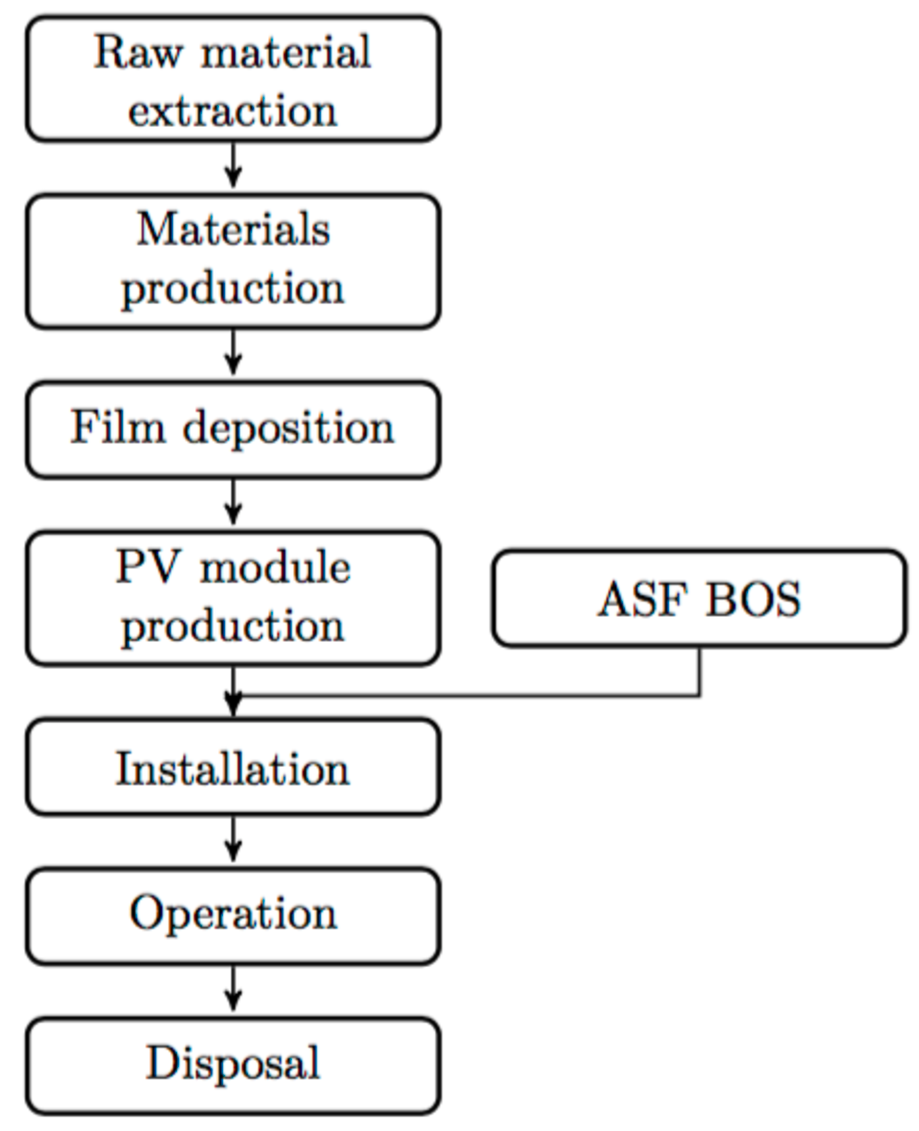
\includegraphics[width=14cm, trim= 0cm 0cm 0cm 0cm,clip]{BOS.pdf}
\caption{Breakdown of the ASF into five embodied product components and installation costs, operational costs, and disposal}
\label{fig:BOS}
\end{center}
\end{figure}

\textcolor{magenta}{\textit{@Zoltan: Should this be pushed to an Annex, or shall we leave it as is}}

\subsubsection*{PV Panel}
\textcolor{magenta}{\textit{(It is nice to explain the inventory step by step, but this will take a lot of space... We might have to reconsider later.)}}
Weight is the primary restriction when selecting a PV panel. Any technology that requires glass encapsulation or a heavy substructure can therefore not be used. This limits us to CIGS and amorphous silicon panels.\\

CIGS PV panels was selected as the thin film panel of choice due to its high efficiency, low cost, and ability to be deposited on a polymer or aluminium substrate \cite{chirilua2011highly}. 

%A less efficient thin film amorphous silicon panel could also be used and will also be discussed in this analysis.\\

\textcolor{magenta}{\textit{(Not sure if it makes sense to provide the entire inventory here. If so, we would probably also need to give expected lifetimes, etc.)}}

% \begin{table}[H]
% \centering
% \begin{tabular}{lll}
% Panel Type  & SMQ    & ${\mathrm{\eta}}$  \\
% \hline
% CIGS 				& 0.7036 ${\mathrm{m^2_{panel}/m^2}}$ & 15\% \\
% a-Si				 	& 0.7036 ${\mathrm{m^2_{panel}/m^2}}$ & YY\%    \\
% Aluminum sheet 		& x ${\mathrm{kg/m^2}}$
% \end{tabular}
% \caption{Possible PV technologies for an ASF [Ref required]}
% \label{tab:PV}
% \end{table}

\begin{table}[H]
\centering
\begin{tabular}{ll}
\hline
CIGS         & xx g/m2 \\
Junction Box &         \\
Power Cables &         \\
\hline
\end{tabular}
\caption{Inventory of main input flows to the PV manufacturing process [ref required]}
\label{tab:PVinv}
\end{table}


\subsubsection*{Actuator}
Traditionally photovoltaic actuation is done through the use of servo motors. Servo motors however become a limiting factor for adaptive facades due to their high upfront costs, and instability in heavy winds. Soft robotic actuators on the other hand are cheaper and more resilient to harsh environmental conditions\cite{Svetozarevic2014a}. The soft robotic actuators however are still in development and have a life time of five years. They will therefore require two rounds of maintenance during the lifetime of the ASF.
For the purpose of this analysis we will analyse both servo motors and soft robotic actuators. \\

\begin{table}[H]
\centering
\begin{tabular}{ll}
\hline
Compressor & xxg/unit  \\
Tubes      & xxgCO2/m  \\
Silicone   & xxgCO2/yy \\
\hline
\end{tabular}
\caption{Inventory of main input flows to the Actuator manufacturing process [ref required]}
\label{tab:ActuatorInv}
\end{table}

\subsubsection*{Cantilever}
The cantilever is a steel connection point between the PV panel and the supporting structure.\\

\begin{table}[H]
\centering
\begin{tabular}{ll}
\hline
Steel & xxgCO2/yy \\
xxxx  & xxgCO2/yy \\
yyyyy & xxgCO2/yy \\
\hline
\end{tabular}
\caption{Inventory of main input flows to the Cantilever manufacturing process [ref required]}
\label{tab:CantileverInv}
\end{table}

\subsubsection*{Supporting Structure}
The supporting structure is the connection point between the array of photovoltaic modules and the building itself. Many different designs are possible, however we will base our analysis of an adaptive solar facade that has already been constructed \cite{nagy2015frontiers}. This design consists of a steel cable-net that spans a steel supporting frame. The steel frame is then attached to the building itself.\\

\begin{table}[H]
\centering
\begin{tabular}{ll}
\hline
Steel & xxgCO2/yy \\
xxxx  & xxgCO2/yy \\
yyyyy & xxgCO2/yy \\
\hline
\end{tabular}
\caption{Inventory of main input flows to the manufacturing process of the Supporting Structure[ref required]}
\label{tab:StructureInv}
\end{table}

\subsubsection*{Controls and Electronic System}
The control system is required for the actuation of panels and the regulation of photovoltaic electricity production.\\

\begin{table}[H]
\centering
\begin{tabular}{ll}
\hline
Steel & xxgCO2/yy \\
xxxx  & xxgCO2/yy \\
yyyyy & xxgCO2/yy \\
\hline
\end{tabular}
\caption{Inventory of main input flows to the manufacturing process of the Control System[ref required]}
\label{tab:ControlInv}
\end{table}

\subsubsection*{Installation}

The installation of the ASF to the building requires a hydraulic hoist which needs to be in operation for eight hours based off previous construction experience \cite{jayathissa2015abs}. \\

\begin{table}[H]
\centering
\begin{tabular}{ll}
\hline
Steel & xxgCO2/yy \\
xxxx  & xxgCO2/yy \\
yyyyy & xxgCO2/yy \\
\hline
\end{tabular}
\caption{Inventory of main input flows to the Assembly Process[ref required]}
\label{tab:AssemblyInv}
\end{table}


\subsection{Operational Emissions and Assumptions}

The potential savings are based off previously completed numerical simulations \cite{jayathissa2015abs}. The simulation was conducted on a south facing office room. The room xx meters in length, xx meters wide and xx meters high was modeled using Rhinoceros 3D CAD Package \cite{Rhino}, shown in Figure XX. Grasshopper \cite{grasshopper} was used to model the dynamic aspects of the ASF which consists of an array of 400mm CIGS solar panels. The geometrical input is imported to Energy Plus \cite{energyplus} though the DIVA \cite{DIVA} interface. A single zone thermal analysis was conducted for each possible geometrical configuration of the ASF for each hour of the year. The results were then post processed in Python \cite{python} with the NumPy \cite{numpy}, and pandas \cite{pandas} plug-ins.\\

Based on the assumption of XX full openings and closings per day, we approximate the energy requirement to actuate the ASF to be YY kWh in its lifetime.\\

\begin{table}[H]
\centering
\begin{tabular}{ll}

\textbf{Building Settings}    &                                                \\
Office Envelope               & Roof: Adiabativ                                \\
                              & Floor: Adiabatic                               \\
                              & Walls: Adiabatic                               \\
                              & Window: Double Glazed LoE (e=0.2) 3mm/13mm air \\
                              & Floor Area: 21.7m2                             \\
Thermal Set Points            & Heating: 22 degrees Celcius                    \\
                              & Cooling: 26 degrees Celcius                    \\
Building System               & Hydronic Heating: COP 4                        \\
                              & Hydronic Cooling: COP3                         \\
Lighting Control              & Lighting set point: 11.8W/m2                   \\
                              & Lighting Control: 300 Lux Threshhold           \\
                              & LED Lighting                                   \\
Occupancy                     & Office: Weekdays from 8:00-18:00               \\
                              & People set point: 0.1 persons/m2               \\
                              & Infiltration: 0.5 per hour                     \\
                              &                                                \\
\textbf{Location Assumptions} &                                                \\
Weather File                  & Geneva, Switzerland (067000IWEC)              \\
Electricity Mix               & ENTSO-E                                           \\
                              &                                                \\
\textbf{Maintenance}          &                                                \\
Actuator Changes              & Every 5 years                                  \\
                              &                                                \\
\textbf{ASF Settings}         &                                                \\
Full open and closes per day  & 3 per day                                      \\
\hline
\end{tabular}
\caption{Summary of main assumptions for the calculation of operational emissions [ref required]\textcolor{magenta}{\textit{(Put me into Annex?)}}}
\label{tab:AssumptionsOpp}
\end{table}


% Maybe have a reference case here, see previous commits 

\subsection{Evaluation Method}
The life cycle analysis is performed according to the ISO 14040 and ISO 14044 guidelines. The analysis is therefore divided into goal and scope definition, inventory analysis, impact assessment and interpretation\\ % 15804 to be discussed

This paper assesses carbon emission reductions, therefore the impact category used is the global warming potential (GWP\textcolor{magenta}{\textit{[IPCC 2013 reference - let me know if you need it]}}). This is described as the emissions of ${\mathrm{CO_2-eq}}$ in kilograms divided by the functional unit. The functional unit needs to be based on the primary function of the technology. For adaptive building integrated photovoltaics this function can be twofold. When the adaptive BIPV acts as a shading system in front of a glass facade area the functional unit of ${\mathrm{m^2}}$ is used, while a comparison with static facade mounted photovoltaic systems requires the functional unit of electricity produced in ${\mathrm{kWh}}$. \textcolor{magenta}{\textit{(We should discuss the functional unit again. It should be defined more precisely / comprehensively.)}}

According to International Energy Agency (IEA) [REF REQUIRED], the calculation of energy (kWh) produced \textcolor{magenta}{\textit{G?}} needs to be based on the conversion efficiency ${\eta}$, performance ratio \textit{PR}, irradiation \textit{I}, lifetime (service life) \textit{LT} and area \textit{A} of the module. Equation \ref{eq:solar} gives the exact formulation:
	
\begin{equation}
G=\frac{{\mathrm{GWP}}}{{\mathrm{I \cdot \eta  \cdot PR \cdot LT \cdot A}}}
% what is G
\label{eq:solar}
\end{equation}

The scope of the LCA comprises of the embodied, operational, and disposal global warming impact of the respective system. Figure \ref{fig:BOS} illustrates the system boundaries of the process flows. The supporting structures are also included in the system boundaries. The reason for this is that technologies within the building envelope also change the design of the supporting structures. The supporting structure of solar panels is referred to as balance of systems (BOS).\\

The inventory data was obtained through technical drawings, research papers describing the technology and expert judgement. The Ecoinvent v3.1 database is used as the main LCI database \cite{frischknecht2005ecoinvent}. To keep assumptions consistent, only data from this database is used. \textcolor{magenta}{\textit{(Is that so? Didn't we add a CIGS dataset?)}} Furthermore, the cut-off approach is used for the allocation of recycling and landfill disposal. This means that recycling does not generate any credit for the product and resulting benefits are not taken into account. Furthermore the use of recycled products do not bear the burden of processes higher up the chain.\textcolor{magenta}{\textit{(We don't do any system expansion?)}}\\

For the impact assessment the ReciPe midpoint (H) indicator is used \cite{zelm2009recipe}. \textcolor{magenta}{\textit{(This is a little inconsistent. We should consistently use the term environmental impact as opposed to carbon content, etc.)}} The impact assessment is performed using the OpenLCA impact assessment tool \cite{ciroth2007ict}.\\
	% we may need to discuss system expansion
	% PV electricity production not included?

% what LCI DB (ecoinvent) is used? refer to Annex?
% see above. Explain what is included and excluded

\textcolor{magenta}{
Things which should be addressed (in more detail):
\begin{itemize}
\item service life of components
\item In case we do a comparative LCA, also the "conventional" system needs to be described.
\item Do we give benefits / credits for injecting electricity into the grid? What is being substituted and how?
\end{itemize}}